%% chapter1_slides.tex
%% Beamer slides for Chapter 1: Introduction
%% "The Krasnosel'skii-Mann Iterative Method: Recent Progress and Applications"
%% by Qiao-Li Dong, Yeol Je Cho, Songnian He, Panos M. Pardalos, Themistocles M. Rassias
%% (SpringerBriefs in Optimization, 2022)
%% Reader-friendly style: complete sentences, symbol explanations, worked examples.
%% Compiled with: pdflatex -interaction=nonstopmode chapter1_slides.tex  (twice)
\documentclass[aspectratio=169,10pt]{beamer}

\usetheme{Madrid}
\usecolortheme{seahorse}
\usefonttheme{professionalfonts}

%% ── Packages ──────────────────────────────────────────────────────────────
\usepackage{amsmath,amssymb,amsfonts}
\usepackage{mathtools}
\usepackage{graphicx}
\usepackage{booktabs}
\usepackage{xcolor}
\usepackage{listings}

\graphicspath{{figures/}}

%% ── Python listing style ─────────────────────────────────────────────────
\lstdefinestyle{pycode}{
  language=Python,
  basicstyle=\ttfamily\scriptsize,
  numbers=left,
  numberstyle=\tiny\color{gray},
  frame=single,
  backgroundcolor=\color{gray!7},
  keywordstyle=\color{blue!70!black}\bfseries,
  commentstyle=\color{green!50!black}\itshape,
  stringstyle=\color{orange!80!black},
  showstringspaces=false,
  breaklines=true,
  tabsize=2,
  xleftmargin=1.0em,
  framexleftmargin=1.0em,
  aboveskip=4pt,
  belowskip=4pt,
}
\lstset{style=pycode}

%% ── Convenience macros ───────────────────────────────────────────────────
\newcommand{\Hil}{\mathcal{H}}
\newcommand{\Fix}{\operatorname{Fix}}
\newcommand{\R}{\mathbb{R}}
\newcommand{\Id}{\mathrm{Id}}

%% ── Metadata ─────────────────────────────────────────────────────────────
\title[KM Method -- Ch.1]{The Krasnosel'ski\u{i}-Mann Iterative Method}
\subtitle{Chapter 1: Introduction}
\author{Based on Dong, Cho, He, Pardalos \& Rassias}
\institute{SpringerBriefs in Optimization, 2022}
\date{}

\setbeamertemplate{footline}[frame number]
\setbeamertemplate{navigation symbols}{}

%% ══════════════════════════════════════════════════════════════════════════
\begin{document}

\begin{frame}
  \titlepage
\end{frame}

\begin{frame}{Chapter Overview}
  \tableofcontents
\end{frame}

%% ══════════════════════════════════════════════════════════════════════════
\section{Notation you'll need}
%% ══════════════════════════════════════════════════════════════════════════

\begin{frame}[allowframebreaks]{Notation and Background You Need}

Before diving in, here is a plain-English glossary of every non-elementary
term used later in this deck. \textbf{We will use $\R^2$ as the concrete
setting for every example}, so nothing here needs to stay abstract.

\begin{itemize}
  \item \textbf{Hilbert space $\Hil$}: think of $\R^n$ generalized to
    possibly infinite dimensions, but keeping the same notion of length and
    angle. Concretely in this deck, $\Hil = \R^2$ with the usual dot product.
  \item \textbf{Inner product $\langle x,y\rangle$}: the ordinary dot
    product $x^{(1)}y^{(1)}+x^{(2)}y^{(2)}$ in $\R^2$; measures ``how much
    two vectors point the same way.''
  \item \textbf{Norm $\|x\|$}: the length of the vector $x$,
    $\|x\|=\sqrt{\langle x,x\rangle}$ (ordinary Euclidean length in $\R^2$).
  \item \textbf{Closed convex set $C$}: a set with no gaps at its boundary
    (closed) such that the straight segment between any two of its points
    stays inside it (convex). Running example: the closed unit disk
    $C=\{x\in\R^2:\|x\|\le 1\}$.

\framebreak

  \item \textbf{Operator / mapping $T:C\to C$}: just a function that takes
    a point of $C$ and returns another point of $C$.
  \item \textbf{Fixed point of $T$}: a point $x$ that $T$ sends to itself,
    $T(x)=x$ -- i.e., a point the map ``leaves alone.'' $\Fix(T)$ denotes
    the set of all fixed points of $T$.
  \item \textbf{Nonexpansive operator}: a map that never increases the
    distance between two points, $\|T(x)-T(y)\|\le\|x-y\|$ for all $x,y$ --
    informally, ``non-stretching.'' It is allowed to preserve distances
    exactly (like a rotation), so it need not pull points together.
  \item \textbf{Contraction}: a \emph{strictly} shrinking map: there is a
    fixed constant $\alpha\in[0,1)$ with $\|T(x)-T(y)\|\le\alpha\|x-y\|$ for
    all $x,y$. Every contraction is nonexpansive, but not conversely
    (a rotation is nonexpansive but not a contraction).
  \item \textbf{Firmly nonexpansive operator}: an even more well-behaved
    special case of nonexpansive, satisfying
    $\|T(x)-T(y)\|^2\le\langle T(x)-T(y),x-y\rangle$. The metric projection
    $P_C$ (below) is always firmly nonexpansive.

\framebreak

  \item \textbf{Metric projection $P_C(x)$}: the closest point of $C$ to
    $x$. In our running example ($C$ = closed unit disk),
    \[
      P_C(x) = \begin{cases} x, & \|x\|\le 1,\\[2pt] x/\|x\|, & \|x\|>1.\end{cases}
    \]
    Geometrically: if $x$ is already inside the disk, leave it alone;
    otherwise, slide it straight in to the nearest boundary point.
  \item \textbf{Banach contraction principle}: if $T$ is a contraction on a
    complete space, it has exactly one fixed point, and repeatedly applying
    $T$ from any starting point converges to it. This is the classical
    engine behind Picard iteration (Section 1.1) -- but it needs
    \emph{strict} shrinking, which nonexpansive maps do not guarantee.
  \item \textbf{Strong vs.\ weak convergence (informal)}: in $\R^n$ these
    coincide, so do not worry about the distinction while thinking in
    $\R^2$; in infinite dimensions they can differ, and the book flags
    which kind of convergence each theorem gives.
\end{itemize}

\end{frame}

%% ══════════════════════════════════════════════════════════════════════════
\section{The fixed point problem}
%% ══════════════════════════════════════════════════════════════════════════

\begin{frame}{Why Fixed Points? The Central Problem}
\small
Many computational questions -- solving equations, finding equilibria,
minimizing a function -- can be rephrased as: \emph{is there a point that a
certain map sends to itself, and how do we find it?} This chapter sets up
that single unifying question.

\begin{block}{The fixed point problem (Eq.\ 1.1)}
Let $\Hil$ be a Hilbert space (reminder: think $\R^n$, generalized), $C$ a
nonempty closed convex subset of $\Hil$, and $T:C\to C$ an operator. Denote
by $\Fix(T)=\{x\in C: x=T(x)\}$ the set of fixed points of $T$.
\[
  \text{Find } x^*\in C \text{ such that } T(x^*)=x^*.
\]
\begin{itemize}
  \item $\Hil$: the ambient space (here, always $\R^2$).
  \item $C$: the region we search in (here, the closed unit disk).
  \item $T$: the map whose fixed points we seek (here, $T=P_C$).
\end{itemize}
\end{block}

This problem has applications in dynamical systems, integral and
differential equations, mathematical economics (game theory, equilibrium
problems), and optimization. Three natural questions arise: (a) does a
fixed point exist? (b) is it unique? (c) if it exists, how do we
\emph{compute} it? This book -- and this chapter -- focus on (c).

\end{frame}

\begin{frame}[allowframebreaks]{Existence and Uniqueness: What Can Go Wrong}

Before building algorithms, it helps to see how differently contractions
and nonexpansive maps behave regarding existence/uniqueness of fixed
points -- this motivates why an entire book is devoted to the nonexpansive
case.

\begin{itemize}
  \item If $T:\Hil\to\Hil$ is a \emph{contraction} (reminder: strictly
    shrinking by a fixed factor $\alpha<1$), the Banach contraction
    principle guarantees \emph{exactly one} fixed point.
  \item If $T$ is merely \emph{nonexpansive} (reminder: non-stretching, but
    not necessarily shrinking), the situation is qualitatively different:
  \begin{itemize}
    \item $T$ may have \textbf{no} fixed point at all: e.g.\ $T(x)=x+z$ for
      a fixed nonzero vector $z$ (a pure translation) is nonexpansive
      ($\|T(x)-T(y)\|=\|x-y\|$ always) but never sends any point to itself.
    \item $T$ may have \textbf{exactly one} fixed point: e.g.\ $T=-\Id$
      (send $x\mapsto -x$) is nonexpansive, and its only fixed point is the
      origin.
    \item $T$ may have \textbf{infinitely many}: e.g.\ $T=\Id$ (the
      identity) fixes every point.
    \item Even \emph{firmly} nonexpansive operators can fail to have a
      fixed point in general infinite-dimensional settings (a subtlety we
      will not need in $\R^2$, since our running example's $T=P_C$ always
      has fixed points -- namely all of $C$ itself).
  \end{itemize}

\framebreak

  \item \textbf{Consequence:} because contractions behave so well
    (existence \emph{and} uniqueness, plus a convergent algorithm for
    free), most of the difficulty -- and most of this book -- concerns the
    \emph{merely nonexpansive} case, where we must work harder both to
    guarantee convergence and to design the right iterative scheme.
\end{itemize}

\end{frame}

%% ══════════════════════════════════════════════════════════════════════════
\section{1.1 Fixed Point Iteration Procedures}
%% ══════════════════════════════════════════════════════════════════════════

\begin{frame}[allowframebreaks]{1.1(A) The Picard Iteration}

The simplest possible idea: just keep applying $T$ over and over, and hope
the results settle down. This is the Picard iteration.

\begin{block}{Picard iteration (Eq.\ 1.2)}
Let $C$ be a nonempty closed convex set of $\Hil$ and $T:C\to C$ a mapping.
For an arbitrary $x_0\in C$, the \emph{Picard iteration} $\{x_n\}$ is
\[
  x_{n+1} = T(x_n) \qquad \text{for each } n\ge 0.
\]
\begin{itemize}
  \item $x_0$: any chosen starting point in $C$.
  \item $x_{n+1}=T(x_n)$: repeatedly ``re-apply $T$'' to the last point.
\end{itemize}
\end{block}

By the Banach contraction principle (notation frame), Picard iteration
\textbf{converges to the unique fixed point whenever $T$ is a contraction}
-- and one even gets explicit error bounds telling you when to stop.

\framebreak

\textbf{The catch:} Picard iteration may fail to produce a fixed point
when $T$ is only nonexpansive (not a contraction). A simple illustration:
$T=-\Id$ (so $T(x)=-x$) and $x_0\ne 0$.

\begin{block}{Worked failure example: $T(x)=-x$, $x_0=(3,4)$}
\begin{itemize}
  \item \textbf{Step 1} (apply $T$ once): $x_1 = T(x_0) = -(3,4) = (-3,-4)$.
  \item \textbf{Step 2} (apply $T$ again): $x_2 = T(x_1) = -(-3,-4) = (3,4) = x_0$.
  \item \textbf{Conclusion}: the sequence just oscillates
    $(3,4),(-3,-4),(3,4),(-3,-4),\dots$ forever -- it never settles down,
    even though $T$ has a (unique) fixed point at the origin
    ($\Fix(T)=\{(0,0)\}$).
\end{itemize}
This is exactly the left panel of the figure below.
\end{block}

\framebreak

\centering

\includegraphics[width=0.85\textwidth]{fig_running_example.pdf}

\vspace{0.3em}
\footnotesize
\textbf{Left:} Picard iteration on the nonexpansive (non-contractive) map
$T(x)=-x$ started at $x_0=(3,4)$: it oscillates forever and never reaches
the fixed point $(0,0)$. \textbf{Right:} the Krasnosel'ski\u{i} iteration
(next slide) on our running example $T=P_C$, started at the same-shaped
point $x_0=(3,4)$, converges smoothly to the fixed point $(0.6,0.8)$.

\end{frame}

\begin{frame}[allowframebreaks]{1.1(B) The Krasnosel'ski\u{i} Iteration}

To rescue Picard iteration for nonexpansive maps, Krasnosel'ski\u{i}
(1955) proposed \emph{damping}: instead of jumping all the way to $T(x_n)$,
move only \emph{halfway} there. Intuition: averaging the current point
with its image under $T$ prevents the oscillation we just saw.

\begin{block}{Krasnosel'ski\u{i} iteration (Eq.\ 1.3)}
\[
  x_{n+1} = \frac{1}{2}x_n + \frac{1}{2}T(x_n) \qquad \text{for each } n\ge 0,
\]
where $x_0\in C$ and $T:C\to C$ is a mapping.
\begin{itemize}
  \item Each new point is the \emph{midpoint} of the current point $x_n$
    and its image $T(x_n)$ -- a ``50/50 blend'' of ``stay put'' and
    ``jump to $T(x_n)$.''
\end{itemize}
\end{block}

\begin{block}{Theorem 1.1 (Krasnosel'ski\u{i})}
Let $X$ be a uniformly convex Banach space and $C$ a convex compact subset
of $X$. If $T:C\to C$ is a nonexpansive mapping with $\Fix(T)\ne\emptyset$,
then $\{x_n\}$ defined by Eq.\ 1.3 converges strongly to a fixed point of
$T$.
\end{block}

\framebreak

Edelstein later weakened ``uniformly convex'' to ``strictly convex.''
Schaefer extended the scheme by replacing the fixed weight $\tfrac12$ with
any constant $\lambda\in(0,1)$:

\begin{block}{General Krasnosel'ski\u{i} iteration (Eq.\ 1.4)}
\[
  x_{n+1} = (1-\lambda)x_n + \lambda T(x_n) \qquad \text{for each } n\ge 0.
\]
\begin{itemize}
  \item $\lambda\in(0,1)$: the (constant) relaxation/damping parameter;
    $\lambda=1$ recovers plain Picard iteration exactly.
\end{itemize}
\end{block}

Schaefer proved weak convergence of Eq.\ 1.4 for a class of continuous
nonexpansive operators. This iteration is exactly the Picard iteration
applied to the \emph{averaged operator}
\[
  T_\lambda = (1-\lambda)\Id + \lambda T,
\]
and one has $\Fix(T)=\Fix(T_\lambda)$ for every $\lambda\in(0,1]$ -- i.e.,
averaging never creates or destroys fixed points, it only changes how fast
(and whether) Picard iteration on $T_\lambda$ converges to one.

\end{frame}

\begin{frame}[allowframebreaks]{Worked Example: Krasnosel'ski\u{i} on Our Running Example}

\textbf{Setup (running example, reused throughout this book's chapters).}
$\Hil=\R^2$, $C=\{x:\|x\|\le 1\}$ (closed unit disk), $T=P_C$ (metric
projection; reminder from the notation frame). Start at $x_0=(3,4)$, and
use $\lambda=\tfrac12$ (Eq.\ 1.3).

\begin{block}{Key observation: everything stays on one ray}
Write $x_0 = 5\cdot(0.6,0.8)$ -- note $(0.6,0.8)$ has norm exactly $1$
(it's already a boundary point of $C$, hence already a fixed point of
$T$). Since $T$ only rescales vectors (it never changes their direction),
every iterate stays on the ray $\{r\cdot(0.6,0.8): r\ge 0\}$. So we can
track just the scalar $r_n$, where $x_n = r_n\cdot(0.6,0.8)$.
\end{block}

As long as $r_n>1$ (point outside the disk), $T(x_n)=x_n/\|x_n\| =
(0.6,0.8)$ exactly (norm-1 point), so the recursion collapses to
\[
  r_{n+1} = \tfrac12 r_n + \tfrac12\cdot 1.
\]

\framebreak

\begin{block}{Step-by-step computation, $r_0=5$}
\begin{itemize}
  \item \textbf{Step 1}: $r_1 = \tfrac12(5) + \tfrac12(1) = 2.5+0.5 = 3$.
  \item \textbf{Step 2}: $r_2 = \tfrac12(3) + \tfrac12(1) = 1.5+0.5 = 2$.
  \item \textbf{Step 3}: $r_3 = \tfrac12(2) + \tfrac12(1) = 1+0.5 = 1.5$.
  \item \textbf{Step 4}: $r_4 = \tfrac12(1.5)+\tfrac12(1) = 0.75+0.5 = 1.25$.
  \item \textbf{Step 5}: $r_5 = \tfrac12(1.25)+\tfrac12(1) = 0.625+0.5=1.125$.
  \item \textbf{Step 6}: $r_6 = \tfrac12(1.125)+\tfrac12(1) = 0.5625+0.5=1.0625$.
  \item \textbf{Pattern}: $r_n - 1 = (r_0-1)\left(\tfrac12\right)^n =
    4\cdot(\tfrac12)^n \to 0$, so $r_n\to 1$ \emph{geometrically}.
\end{itemize}
\end{block}

\textbf{Conclusion:} $x_n = r_n\cdot(0.6,0.8) \to (0.6,0.8)$, the unique
fixed point of $T$ on this ray -- exactly the right panel of the figure on
the previous frame. Contrast with $T=-\Id$: plain Picard ($\lambda=1$)
never converges, but damping with $\lambda<1$ fixes this completely (in
fact, applying Eq.\ 1.3 to $T=-\Id$ from $x_0=(3,4)$ gives
$x_1=\tfrac12(3,4)+\tfrac12(-3,-4)=(0,0)$ -- the fixed point, in a single
step!).

\end{frame}

\begin{frame}[fragile]{Python: Picard Failure vs.\ Krasnosel'ski\u{i} Success}

\begin{lstlisting}
import numpy as np
def project_disk(x):                        # T = P_C
    n = np.linalg.norm(x)
    return x if n <= 1.0 else x / n

x0 = np.array([3.0, 4.0])
x = x0.copy(); picard_trace = [x.copy()]     # Picard on T(x) = -x
for _ in range(4):
    x = -x
    picard_trace.append(x.copy())
print("Picard on T=-Id:", [tuple(p) for p in picard_trace])

lam = 0.5
x = x0.copy(); km_trace = [x.copy()]         # Krasnoselskii on T = P_C
for _ in range(6):
    x = (1 - lam) * x + lam * project_disk(x)      # Eq. 1.3
    km_trace.append(x.copy())
for n, p in enumerate(km_trace):
    print(f"r_{n} = {np.linalg.norm(p):.4f}   x_{n} = ({p[0]:.4f}, {p[1]:.4f})")
\end{lstlisting}

\medskip
\textbf{Output (excerpt):}
\texttt{Picard on T=-Id: [(3,4), (-3,-4), (3,4), (-3,-4), (3,4)]} (never
converges), and \texttt{r\_0=5.0000 ... r\_6=1.0625}, matching the
hand computation exactly.

\end{frame}

\begin{frame}[allowframebreaks]{1.1(B$'$) The Krasnosel'ski\u{i}--Mann (``Mann'') Iteration}

The constant weight $\lambda$ can itself be replaced by a whole
\emph{sequence} $\lambda_n$, allowed to change at every step. This most
general averaging scheme is due to Mann, and the resulting family of
methods is now called the Krasnosel'ski\u{i}--Mann iteration.

\begin{block}{Krasnosel'ski\u{i}--Mann iteration (Eq.\ 1.5)}
\[
  x_{n+1} = (1-\lambda_n)x_n + \lambda_n T(x_n) \qquad \text{for each } n\ge 0,
\]
where $\{\lambda_n\}\subset[0,1]$.
\begin{itemize}
  \item $\lambda_n$: the relaxation parameter \emph{at step $n$} -- no
    longer required to be constant. Choosing $\lambda_n\equiv\lambda$
    recovers Eq.\ 1.4; choosing $\lambda_n\equiv 1$ recovers Picard.
\end{itemize}
\end{block}

This scheme (Eq.\ 1.5) has been studied in a great many papers over the
last sixty years. It is the central object of Chapter 3 of this book.

\framebreak

\textbf{Illustration with our rotation toy example.} To compare Picard,
constant-$\lambda$ Krasnosel'ski\u{i}, and diminishing-step Mann
\emph{on the same simple problem} (our disk-projection $T=P_C$ makes
Picard converge trivially in one step, so it doesn't showcase the
contrast), use instead $T(x,y)=(-y,x)$ -- a $90^\circ$ rotation in
$\R^2$. It is nonexpansive (a rotation never changes lengths) with unique
fixed point $\Fix(T)=\{(0,0)\}$.
\begin{itemize}
  \item \textbf{Picard} ($\lambda_n\equiv1$): from $x_0=(3,4)$, iterates
    cycle around the circle of radius $5$ forever -- $(3,4)\to(-4,3)\to
    (-3,-4)\to(4,-3)\to(3,4)\to\cdots$ -- never converging.
  \item \textbf{Krasnosel'ski\u{i}} ($\lambda_n\equiv\tfrac12$): spirals
    into the origin \emph{geometrically}, shrinking by a factor
    $1/\sqrt2\approx0.707$ every step (the fastest possible rate for this
    example, as shown two slides ahead).
  \item \textbf{Mann} ($\lambda_n=1/(n+2)\to 0$): also spirals into the
    origin, but more slowly, since the damping weakens as $n$ grows.
\end{itemize}

\framebreak

\centering
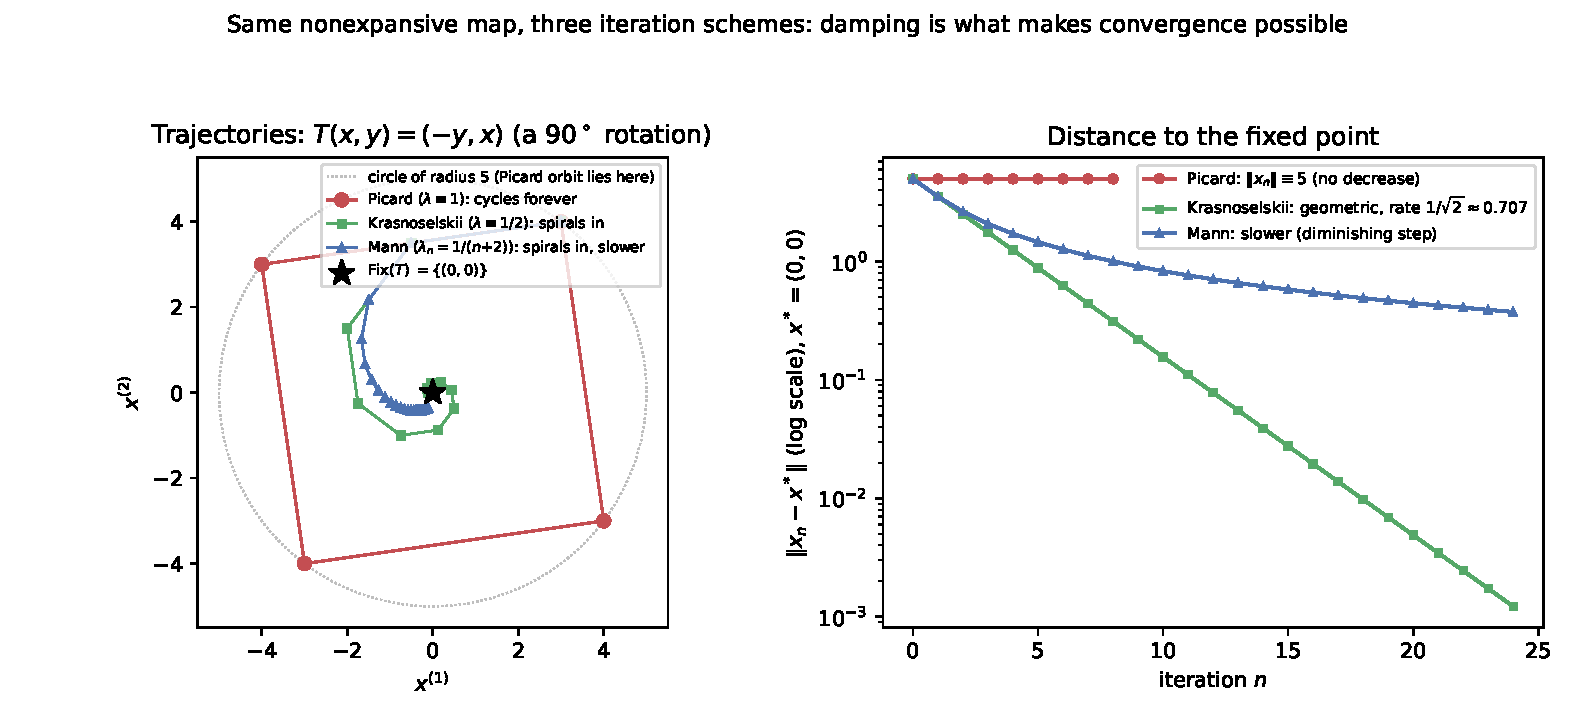
\includegraphics[width=0.78\textwidth]{fig_iteration_comparison.pdf}

\footnotesize
Same nonexpansive map $T(x,y)=(-y,x)$, three schemes, same start
$x_0=(3,4)$. \textbf{Left:} trajectories in the plane. \textbf{Right:}
distance to the fixed point $(0,0)$ versus iteration number (log scale) --
Picard never shrinks, Krasnosel'ski\u{i} shrinks geometrically fastest,
Mann's diminishing steps shrink more slowly but still converge.

\end{frame}

\begin{frame}{Why $\lambda=1/2$ Is Special Here: Rate vs.\ Relaxation Parameter}
\footnotesize
For the rotation example, one can compute exactly how fast the
constant-$\lambda$ averaged map $T_\lambda=(1-\lambda)\Id+\lambda T$
contracts, as a function of $\lambda$.

\begin{block}{Contraction rate of $T_\lambda$ for a $90^\circ$ rotation}
Representing $\R^2$ as the complex plane ($T$ = multiplication by $i$),
$T_\lambda$ multiplies by $(1-\lambda)+\lambda i$, whose modulus is the
contraction rate: $\text{rate}(\lambda) = \sqrt{(1-\lambda)^2+\lambda^2}$.
\begin{itemize}
  \item At $\lambda=1$ (Picard): $\text{rate}=1$ -- no contraction at all,
    consistent with the never-ending cycle we saw.
  \item At $\lambda=0$: $\text{rate}=1$ too (the map never moves).
  \item Minimized at $\lambda=1/2$: $\text{rate}=1/\sqrt2\approx0.707$ --
    exactly Krasnosel'ski\u{i}'s original, historically first choice!
\end{itemize}
\end{block}

\vspace{-0.3em}
\centering
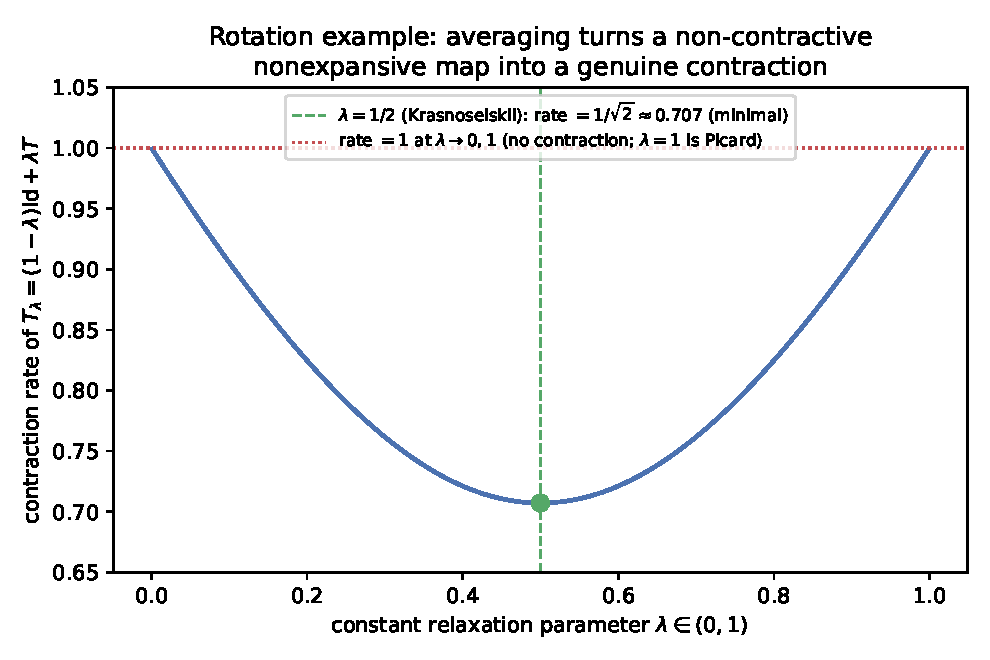
\includegraphics[width=0.42\textwidth]{fig_lambda_rate.pdf}

\end{frame}

\begin{frame}[allowframebreaks]{1.1(C) The Ishikawa Iteration}

Sometimes one averaging step per iteration is not enough to guarantee
convergence for harder classes of maps (beyond nonexpansive). The
Ishikawa iteration adds a \emph{second}, inner averaging step before the
outer update.

\begin{block}{Ishikawa iteration (Eq.\ 1.6)}
For an arbitrary $x_0\in C$, define $\{x_n\}$ by: for each $n\ge 0$,
\[
  \begin{cases}
    y_n = (1-\alpha_n)x_n + \alpha_n T(x_n),\\
    x_{n+1} = (1-\lambda_n)x_n + \lambda_n T(y_n).
  \end{cases}
\]
\begin{itemize}
  \item $y_n$: an \emph{inner} Krasnosel'ski\u{i}-type averaging step,
    with its own parameter $\alpha_n$.
  \item $x_{n+1}$: the \emph{outer} update, applying $T$ to $y_n$ (instead
    of directly to $x_n$) and averaging with weight $\lambda_n$.
  \item This is sometimes called the \emph{two-step} Krasnosel'ski\u{i}--Mann
    iteration.
\end{itemize}
\end{block}

The Ishikawa iteration was first used to establish strong convergence to a
fixed point for a Lipschitz and \emph{pseudocontractive} self-map of a
convex compact subset $C$ of a Hilbert space -- a broader class of maps
than nonexpansive ones, for which the plain Krasnosel'ski\u{i}--Mann
iteration (Eq.\ 1.5) is known to fail (Chidume--Mutangadura built an
explicit counterexample).

\framebreak

\textbf{Trade-offs to keep in mind:}
\begin{itemize}
  \item The Ishikawa iteration is computationally \emph{more expensive}
    per step than Krasnosel'ski\u{i}--Mann (it evaluates $T$ at $y_n$, an
    extra averaged point).
  \item Its convergence \emph{rate} is known to be \emph{slower} than that
    of Krasnosel'ski\u{i}--Mann when both apply.
  \item \textbf{Practical rule of thumb:} when several iterative schemes
    are known to converge for your class of maps, prefer the simplest
    one -- which is usually Krasnosel'ski\u{i}--Mann.
\end{itemize}

\end{frame}

\begin{frame}{Weak vs.\ Strong Convergence: Why We Need Modifications}

In infinite-dimensional spaces (unlike $\R^n$, where the two notions
coincide -- reminder from the notation frame), the Krasnosel'ski\u{i}--Mann
and Ishikawa iterations are generally only guaranteed to converge
\emph{weakly}.

\begin{itemize}
  \item Genel and Lindenstraus constructed a celebrated counterexample: a
    \emph{contractive} operator on a bounded closed convex subset of a
    Hilbert space for which the Krasnosel'ski\u{i} iteration does
    \textbf{not} converge strongly.
  \item Another counterexample exists for the Picard iteration applied to
    the \emph{composition of two projections}.
  \item Yet strong convergence is often much more desirable in
    applications than weak convergence.
\end{itemize}

\medskip
\textbf{Two remedies pursued in the literature (and in this book):}
\begin{enumerate}
  \item \textbf{Additional conditions on $T$} -- e.g., if $T$ is
    \emph{demicontractive} and $\Id-T$ maps closed bounded subsets of $C$
    onto closed subsets of $C$ (in particular if $T$ is demicompact), then
    Eq.\ 1.5 converges \emph{strongly}. Maruster gave another sufficient
    condition: existence of $h\ne 0$ with $\langle x-T(x),h\rangle\le 0$
    for all $x\in C$.
  \item \textbf{Modifications of the iteration itself} -- the Halpern
    iteration and the hybrid (``CQ'') methods, covered next.
\end{enumerate}

\end{frame}

\begin{frame}[allowframebreaks]{1.1(D) The Halpern Iteration}

Idea: instead of averaging $x_n$ with $T(x_n)$, average a \emph{fixed
anchor point} $u$ with $T(x_n)$. Intuition: $u$ acts like a ``magnet''
that pulls the whole sequence toward the fixed point of $T$ that is
\emph{closest to $u$}, which is exactly what buys us strong convergence.

\begin{block}{Halpern iteration (Eq.\ 1.7)}
For any fixed $u\in C$ and arbitrary $x_0\in C$:
\[
  x_{n+1} = \lambda_n u + (1-\lambda_n)T(x_n) \qquad \text{for each } n\ge 0,
\]
where $\{\lambda_n\}\subset[0,1]$ and the convex combination is
``anchored'' to $u$.
\begin{itemize}
  \item $u$: a fixed, chosen ``anchor'' point in $C$ (not updated).
  \item $\lambda_n$: the weight on the anchor at step $n$ (typically
    $\to 0$, so the anchor's pull weakens over time but never vanishes in
    total, per the conditions below).
\end{itemize}
\end{block}

\begin{block}{Standard conditions on $\{\lambda_n\}$}
\begin{itemize}
  \item[(C1)] $\lim_{n\to\infty}\lambda_n = 0$;
  \item[(C2)] $\sum_{n=0}^\infty \lambda_n = \infty$;
  \item[(C3)] $\sum_{n=0}^\infty|\lambda_{n+1}-\lambda_n|<\infty$, or
    $\lim_{n\to\infty}\lambda_n/\lambda_{n+1}=1$.
\end{itemize}
\end{block}

\framebreak

\textbf{Convergence guarantee.} If $T:C\to C$ is nonexpansive with
$\Fix(T)\ne\emptyset$ and $\{\lambda_n\}$ satisfies (C1)--(C3), then
$\{x_n\}$ from Eq.\ 1.7 converges \emph{strongly} to $P_{\Fix(T)}u$ --
i.e., the point of $\Fix(T)$ \emph{closest to the anchor $u$} (reminder:
$P_K$ denotes metric projection onto $K$).

\begin{block}{A tight, quantitative convergence-rate bound}
With the popular choice $\lambda_n=\tfrac1{n+2}$ and $u=x_0$:
\[
  \|x_n-T(x_n)\| \le \frac{2\|x_0-x^*\|}{n+1}
  \qquad \text{for each } n\ge 1 \text{ and } x^*\in\Fix(T).
\]
\begin{itemize}
  \item Left side: how far the current iterate is from being a fixed
    point (a computable ``residual'').
  \item Right side: an explicit $O(1/n)$ bound, entirely in terms of the
    starting distance to \emph{any} fixed point $x^*$.
\end{itemize}
\end{block}

The convergence speed of the Halpern iteration is widely believed to be
slow, due to the strict restriction (C2). Later work found improved,
data-driven choices of $\{\lambda_n\}$ (Eq.\ 1.8 in the book) that speed
this up substantially in practice -- we omit the lengthy closed form here
and refer to it only by name.

\framebreak

\textbf{A useful special case: minimum-norm fixed points.} Taking $u=0$ in
Eq.\ 1.7 targets $P_{\Fix(T)}(0)$, the fixed point of $T$ closest to the
origin -- of independent interest in convex optimization. But if $0\notin
C$, the naive analogue
\[
  x_{n+1} = (1-\lambda_n)T(x_n)
\]
can leave $C$ entirely (since it drops the anchor term), so it cannot be
used directly. Two fixes appear in the literature:
\begin{itemize}
  \item \textbf{Project back into $C$} after each step (Wang--Xu, Eq.\
    1.9): $x_{n+1}=P_C[(1-\lambda_n)T(x_n)]$ -- correct, but often hard to
    implement because $P_C$ itself may have no closed form.
  \item \textbf{An explicit boundary-point algorithm} (He et al.):
    define $h(x)=\inf\{\lambda\in(0,1]:\lambda x\in C\}$ for $x\in C$
    (Eq.\ 1.10) -- ``how much must we shrink $x$ toward the origin to
    land exactly on the boundary of $C$ (through the origin's direction)?''
    -- and iterate
    \[
      x_{n+1} = \lambda_n\theta_n x_n + (1-\lambda_n)T(x_n), \qquad
      \theta_n = h(x_n)
    \]
    (Eq.\ 1.11), which converges strongly to $P_{\Fix(T)}(0)$ under mild
    conditions on $\{\lambda_n\},\{\theta_n\}$ (Theorem 1.2). The main
    practical difficulty is computing $h$ in closed form; this is doable,
    e.g., when $C$ is defined by a single quadratic inequality.
\end{itemize}

\end{frame}

\begin{frame}[allowframebreaks]{1.1(E) The Viscosity Iteration}

Moudafi extended the Halpern iteration by replacing the \emph{fixed}
anchor $u$ with a \emph{moving} anchor $f(x_n)$, where $f$ is a
contraction -- like a ``brake'' riding along with the current iterate
rather than a single fixed magnet.

\begin{block}{Viscosity iteration (Eq.\ 1.12)}
\[
  x_{n+1} = \lambda_n f(x_n) + (1-\lambda_n)T(x_n) \qquad \text{for each } n\ge 0,
\]
where $f:C\to C$ is a contraction (reminder: strictly shrinking by a fixed
factor $<1$).
\begin{itemize}
  \item $f$: the ``viscosity'' term -- replaces the constant anchor $u$ of
    Halpern's scheme with a contraction applied to the current iterate.
  \item Setting $f\equiv u$ (a constant map) recovers the Halpern
    iteration exactly.
\end{itemize}
\end{block}

\begin{block}{Theorem 1.3 (Xu)}
Let $T:C\to C$ be nonexpansive with $\Fix(T)\ne\emptyset$ and $f:C\to C$ a
contraction with constant $\alpha\in[0,1)$. Under conditions (C1)--(C3) on
$\{\lambda_n\}$, the sequence $\{x_n\}$ from Eq.\ 1.12 converges strongly
to the unique solution $q\in\Fix(T)$ of the variational inequality
\[
  \langle f(q)-q,\, x-q\rangle \le 0 \qquad \text{for all } x\in\Fix(T).
\]
\end{block}

\framebreak

\begin{itemize}
  \item Why is this variational inequality solvable uniquely? Because
    $\Id-f$ turns out to be $(1+\alpha)$-Lipschitz and
    $(1-\alpha)$-strongly monotone (formal definitions come in Chapter 2;
    intuitively, $\Id-f$ is well-behaved enough to guarantee a unique
    solution).
  \item The introduction of the viscosity term is not just cosmetic: it
    lets the limit point depend on $f$ (not only on the geometry of
    $\Fix(T)$), which is exploited heavily in applications (e.g., to select
    a specific, ``regularized'' fixed point).
  \item Many further extensions and generalizations of Eq.\ 1.12 exist in
    the literature; He et al.\ also gave optimal choices of $\{\lambda_n\}$
    for this scheme, analogous to Eq.\ 1.8 for Halpern's iteration.
\end{itemize}

\end{frame}

\begin{frame}{1.1(E$'$) The Regularized Krasnosel'ski\u{i}--Mann Iteration}

Yao et al.\ introduced a variant that regularizes the \emph{current point}
itself (rather than adding an anchor or viscosity term), by shrinking it
toward the origin before applying $T$.

\begin{block}{Regularized Krasnosel'ski\u{i}--Mann iteration (Eq.\ 1.14)}
For $T:\Hil\to\Hil$ nonexpansive: for each $n\ge 0$,
\[
  \begin{cases}
    y_n = \beta_n x_n,\\
    x_{n+1} = (1-\lambda_n)y_n + \lambda_n T(y_n),
  \end{cases}
\]
with $\{\lambda_n\},\{\beta_n\}\subset[0,1]$.
\begin{itemize}
  \item $y_n=\beta_n x_n$: shrinks $x_n$ toward the origin by factor
    $\beta_n$ \emph{before} averaging with $T(y_n)$.
\end{itemize}
\end{block}

\begin{block}{Theorem 1.4 (Bo\c t et al., improving on Yao et al.)}
If $\{\lambda_n\},\{\beta_n\}$ satisfy: $0<\beta_n\le1$,
$\lim_n\beta_n=1$, $\sum_n(1-\beta_n)=\infty$,
$\sum_n|\beta_n-\beta_{n-1}|<\infty$; and $0<\lambda_n\le1$,
$\liminf_n\lambda_n>0$, $\sum_n|\lambda_n-\lambda_{n-1}|<\infty$; then
$\{x_n\}$ converges \emph{strongly} to $P_{\Fix(T)}(0)$ -- the minimum-norm
fixed point, obtained here \emph{without} needing anchor points or
explicit projections.
\end{block}

\end{frame}

\begin{frame}[allowframebreaks]{1.1(F) The Hybrid Methods (the ``CQ'' Algorithm)}

A completely different strategy for forcing strong convergence: at each
step, build two auxiliary closed convex sets $C_n$ (``don't retreat from
the target'') and $Q_n$ (``stay consistent with your history''), then
\emph{project the original starting point $x_0$} onto their intersection.
Independently proposed in Haugazeau's unpublished dissertation, and later
combined with the Krasnosel'ski\u{i}--Mann iteration by Nakajo and
Takahashi.

\begin{block}{The Nakajo--Takahashi hybrid (``CQ'') algorithm (Eq.\ 1.15)}
$x_0\in C$ chosen arbitrarily; for each $n\ge0$,
\[
  \begin{cases}
    y_n = \lambda_n x_n + (1-\lambda_n)T(x_n),\\
    C_n = \{z\in C: \|y_n-z\|\le\|x_n-z\|\},\\
    Q_n = \{z\in C: \langle x_n-z,\,x_n-x_0\rangle\le 0\},\\
    x_{n+1} = P_{C_n\cap Q_n}\,x_0.
  \end{cases}
\]
\begin{itemize}
  \item $y_n$: an ordinary Krasnosel'ski\u{i}--Mann step from $x_n$.
  \item $C_n$: the set of points \emph{at least as close to $y_n$ as
    $x_n$ is} -- a ``don't get farther from the fixed point candidate''
    constraint.
  \item $Q_n$: a half-space built from the history of the iteration,
    separating $x_0$ from ``already-explored'' territory.
  \item $x_{n+1}$: re-project the \emph{original} $x_0$ onto
    $C_n\cap Q_n$ -- this is what is often called the \emph{CQ algorithm}.
\end{itemize}
\end{block}

\framebreak

\textbf{Convergence.} If $T:C\to C$ is nonexpansive with
$\Fix(T)\ne\emptyset$ and $\{\lambda_n\}\subset[0,\sigma]$ for some
$\sigma\in[0,1)$, then $x_n\to P_{\Fix(T)}(x_0)$ \emph{strongly} -- under
strictly weaker conditions on $\{\lambda_n\}$ than the Halpern iteration
needs.

\textbf{A family of further refinements.} Since Eq.\ 1.15, many
modifications have been proposed; the book highlights three:

\begin{itemize}
  \item \textbf{Shrinking projection method} (Eq.\ 1.16): start with
    $C_1=C$, $x_1=P_{C_1}x_0$, and for $n\ge0$,
  \[
    y_n=\lambda_n x_n+(1-\lambda_n)T_n(x_n), \quad
    C_{n+1}=\{z\in C_n:\|y_n-z\|\le\|x_n-z\|\}, \quad
    x_{n+1}=P_{C_{n+1}}x_0.
  \]
    Here $C_n$ \emph{shrinks} monotonically (a half-space is intersected
    in at every step), which limits practical use for large $n$.

\framebreak

  \item \textbf{An efficient numerical variant} (Eq.\ 1.17): with
    $x_0,z_0\in C$ arbitrary and $\lambda_n\in[0,\sigma]$,
    $\sigma\in[0,\tfrac12)$,
  \[
    z_{n+1}=\lambda_n z_n+(1-\lambda_n)T(x_n), \quad
    C_n=\{z\in C:\|z_{n+1}-z\|^2\le\alpha_n\|z_n-z\|^2+(1-\alpha_n)\|x_n-z\|^2\},
  \]
    with $Q_n$ exactly as in Eq.\ 1.15 and $x_{n+1}=P_{C_n\cap Q_n}x_0$.

  \item \textbf{The main practical bottleneck}: computing
    $x_{n+1}=P_{C_n\cap Q_n}x_0$ is, in general, itself a nontrivial
    optimization problem -- despite many papers studying hybrid methods
    theoretically, very few give a way to actually \emph{compute} the
    projection efficiently.

\framebreak

  \item \textbf{An explicit realization when $C=\Hil$} (He et al., Eq.\
    1.18): defines $u_n=\tfrac12(x_n+y_n)$ and half-spaces
    $C_n=\{z:\langle x_n-u_n,z-u_n\rangle\le0\}$,
    $Q_n=\{z:\langle x_0-x_n,z-x_n\rangle\le0\}$, for which
    $P_{C_n\cap Q_n}x_0$ can be written down in closed form (via two
    auxiliary points $z_n,w_n$ built from inner products of the current
    data) -- avoiding any numerical optimization subproblem entirely.
  \item \textbf{A further variant for general $C$} (He--Yang, Eq.\ 1.19):
    combines Eq.\ 1.15's $C_n,Q_n$ with an \emph{extra} projection back
    onto $C$ at the end,
    $u_{n+1}=P_{C_n\cap Q_n}x_0$, $x_{n+1}=P_C\,u_{n+1}$, which is
    sometimes easier to compute when $C$ has simple structure (e.g., a
    ball or a box) even though $C_n\cap Q_n$ does not.
\end{itemize}

\framebreak

\textbf{Takeaway for this section.} We now have an entire toolbox of
schemes -- Picard, Krasnosel'ski\u{i}, (Krasnosel'ski\u{i}--)Mann,
Ishikawa, Halpern, viscosity, regularized, and hybrid/CQ -- trading off
simplicity, computational cost per step, and the strength of convergence
(weak vs.\ strong) they guarantee. Chapters 3--7 of the book dig deeply
into refinements of exactly this family.

\end{frame}

%% ══════════════════════════════════════════════════════════════════════════
\section{1.2 Fixed Point Formulation of Typical Problems}
%% ══════════════════════════════════════════════════════════════════════════

\begin{frame}{1.2 Overview: Many Problems Are Secretly Fixed Point Problems}

The reason the fixed point problem (Eq.\ 1.1) matters so much is that a
huge variety of classical problems -- nonlinear equations, equilibrium
problems, optimization problems, integral and differential equations --
can all be \emph{rewritten} as ``find $x^*$ with $T(x^*)=x^*$'' for a
suitable operator $T$. Once rewritten, every iteration scheme from
Section 1.1 becomes available to solve them.

\begin{block}{Our running example is already an instance of this}
Finding the projection $P_C(x_0)$ of a point $x_0$ onto a closed convex
set $C$ (as in $C=$ unit disk, $x_0=(3,4)$) is \emph{by definition} the
fixed point problem for $T=P_C$: any $x^*\in C$ with $P_C(x_0)$ landing
back on itself. Since $\Fix(P_C)=C$ always, ``is $x_0$ (or its projection)
in $C$?'' is exactly a tiny \emph{convex feasibility problem}: find some
point in the (nonempty, closed, convex) set $C$. We revisit this
explicitly after introducing variational inequalities below.
\end{block}

\end{frame}

\begin{frame}[allowframebreaks]{1.2(A) The Nonlinear Equation}

\begin{block}{Nonlinear equation (Eq.\ 1.20)}
\[
  F(x) = 0,
\]
where $F:C\subseteq\R^n\to\R^n$ is a given operator.
\begin{itemize}
  \item Finding roots of $F$ is fundamental in numerical mathematics; in
    general one cannot solve Eq.\ 1.20 directly and must resort to
    iterative methods.
\end{itemize}
\end{block}

\textbf{The trick:} rewrite Eq.\ 1.20 \emph{equivalently} as the fixed
point problem $T(x)=x$ for some operator $T$ built from $F$ (called the
\emph{iteration function}). For real, single-variable $F$, the most
popular choice is Newton's method:

\begin{block}{Newton's iteration function (Eq.\ 1.21)}
\[
  T(x) = x - \frac{F(x)}{F'(x)}.
\]
\begin{itemize}
  \item A fixed point of $T$ (where $x=T(x)$) forces $F(x)/F'(x)=0$, i.e.\
    $F(x)=0$ (assuming $F'(x)\ne 0$) -- exactly a root of $F$.
  \item Running Picard iteration on \emph{this} $T$ is precisely Newton's
    method for root-finding.
\end{itemize}
\end{block}

\framebreak

\begin{block}{Theorem 1.5: a whole family of higher-order methods}
Set $F_1=F$ and, recursively for $m\ge2$,
\[
  F_m(x) := \frac{F_{m-1}(x)}{[F_{m-1}'(x)]^{1/m}}.
\]
Then
\[
  G_m(x) = x - \frac{F_{m-1}(x)}{F_{m-1}'(x)}
\]
defines an iteration function whose order of convergence, for simple
roots, is $m$.
\begin{itemize}
  \item $m=2$: $G_2 = T$ from Eq.\ 1.21 (Newton's method, order 2).
  \item $m=3$: $G_3(x) = x - \dfrac{F(x)F'(x)}{F'^2(x)-\tfrac12 F(x)F''(x)}$
    -- this is the iteration function of \emph{Halley's method} (cubic,
    i.e.\ order-3 convergence).
\end{itemize}
\end{block}

\end{frame}

\begin{frame}[fragile]{Python: Newton's Method as a Fixed Point Iteration}

We solve $F(x)=x^2-2=0$ (root $\sqrt2$) by running Picard iteration on
Newton's iteration function $T(x)=x-F(x)/F'(x)$ from Eq.\ 1.21.

\begin{lstlisting}
def F(x):  return x**2 - 2
def Fp(x): return 2*x

def T_newton(x):                # Eq. 1.21: Newton's iteration function
    return x - F(x) / Fp(x)

x = 1.0                         # x0, arbitrary starting guess
for n in range(6):
    print(f"x_{n} = {x:.10f},  F(x_{n}) = {F(x):.2e}")
    x = T_newton(x)              # Picard iteration on T = Newton's map
print(f"x_6 = {x:.10f}   (true sqrt(2) = {2**0.5:.10f})")
\end{lstlisting}

\medskip
\textbf{Output (excerpt):} \texttt{x\_0 = 1.0000000000}, \texttt{x\_1 =
1.5000000000}, \texttt{x\_2 = 1.4166666667}, \texttt{x\_3 =
1.4142156863}, \texttt{x\_4 = 1.4142135624} -- already correct to 9
decimal digits by step 4, illustrating the quadratic convergence rate
promised by Theorem 1.5 with $m=2$.

\end{frame}

\begin{frame}[allowframebreaks]{1.2(B) The Equilibrium Problem}

Many classical existence results predate, and motivate, the modern
equilibrium-problem framework.

\begin{block}{Theorem 1.6 (Hartman--Stampacchia, 1966)}
Let $C$ be a compact convex subset of $\R^n$ and $f:C\to\R^n$ continuous.
Then there exists $x_0\in C$ such that
\[
  \langle f(x_0),\,y-x_0\rangle \ge 0 \qquad \text{for all } y\in C.
\]
\end{block}

\begin{block}{Theorem 1.7 (Ky Fan's best approximation theorem, 1969)}
Let $C$ be a nonempty compact convex set in a normed vector space $E$.
Then, for any continuous $f:C\to E$, there exists $x_0\in C$ such that
\[
  \|x_0-f(x_0)\| = \min_{y\in C}\|y-f(x_0)\|.
\]
In particular, if $f(C)\subset C$, then $x_0$ is a fixed point of $f$.
\end{block}

These two results underlie variational inequalities, complementarity
problems, optimization, and game theory.

\framebreak

\begin{block}{The equilibrium problem, EP (Blum--Oettli, 1994)}
Let $E$ be a normed vector space, $C\subseteq E$ nonempty convex, and
$f:C\times C\to\R$ a bifunction (a function of two arguments). The
\emph{equilibrium problem} is:
\[
  \text{Find } x_0\in C \text{ such that } f(x_0,y)\ge 0 \text{ for all } y\in C.
\]
\begin{itemize}
  \item $f(x,y)$: a ``comparison'' between candidate points $x,y\in C$;
    intuitively, $x_0$ is an equilibrium if no $y$ ``improves on'' $x_0$.
\end{itemize}
\end{block}

\textbf{Standing assumptions on $f$ (for the Hilbert-space theory below),
for all $x,y,z\in C$:}
\begin{itemize}
  \item[(a1)] $f(x,x)=0$;
  \item[(a2)] $f(x,y)+f(y,x)\le 0$ (\emph{monotonicity});
  \item[(a3)] $\displaystyle\lim_{t\to0}f(zt+(1-t)x,y)\le f(x,y)$;
  \item[(a4)] $y\mapsto f(x,y)$ is convex and lower semicontinuous, for
    each fixed $x$.
\end{itemize}

\framebreak

\begin{block}{Lemma 1.1 (existence of an approximate equilibrium)}
Let $f$ satisfy (a1)--(a4), $r>0$, $x\in\Hil$. Then there exists $z\in C$
such that
\[
  f(z,y) + \frac{\langle y-z,\,z-x\rangle}{r} \ge 0 \qquad \text{for all } y\in C.
\]
\end{block}

\begin{block}{Lemma 1.2 (the resolvent $T_r$ of an equilibrium bifunction)}
Under (a1)--(a4), for $r>0$ and $x\in\Hil$, define
\[
  T_r(x) = \left\{z\in C: f(z,y)+\frac{\langle y-z,z-x\rangle}{r}\ge 0
  \ \text{ for all } y\in C\right\}.
\]
Then: (1) $T_r$ is single-valued; (2) $T_r$ is firmly nonexpansive
(reminder: $\|T_r(x)-T_r(y)\|^2\le\langle T_r(x)-T_r(y),x-y\rangle$); (3)
$\Fix(T_r)=EP(f)$; (4) $EP(f)$ (the solution set of the equilibrium
problem) is nonempty, closed, and convex.
\end{block}

\framebreak

\textbf{Why this matters for us:} Lemma 1.2 says solving the equilibrium
problem is \emph{literally} a fixed point problem for the (firmly
nonexpansive!) resolvent operator $T_r$ -- so every scheme from Section
1.1 (Krasnosel'ski\u{i}--Mann, Halpern, viscosity, hybrid methods, \dots)
applies directly.

\end{frame}

\begin{frame}[allowframebreaks]{1.2(B$'$) Special Cases of the Equilibrium Problem}

The equilibrium problem is a common ``meta-format'' for several
well-known problems: pick the right bifunction $f$, and each becomes a
special case of EP (and hence of the fixed point problem, via $T_r$).

\begin{block}{(1) The minimization problem (MP)}
Find $x\in C$ such that $\phi(x)\le\phi(y)$ for all $y\in C$, where
$\phi:C\to\R$.
\begin{itemize}
  \item Set $f(x,y)=\phi(y)-\phi(x)$: then EP $\equiv$ MP exactly (an
    equilibrium is precisely a global minimizer of $\phi$).
\end{itemize}
\end{block}

\begin{block}{(2) The saddle point problem (SPP)}
Find $(\bar x_1,\bar x_2)\in C_1\times C_2$ such that
$L(\bar x_1,y_2)\le L(\bar x_1,\bar x_2)\le L(y_1,\bar x_2)$ for all
$(y_1,y_2)\in C_1\times C_2$, where $L:C_1\times C_2\to\R$.
\begin{itemize}
  \item Set $C=C_1\times C_2$ and
    $f((x_1,x_2),(y_1,y_2))=L(y_1,x_2)-L(x_1,y_2)$: then EP $\equiv$ SPP.
\end{itemize}
\end{block}

\framebreak

\begin{block}{(3) The Nash equilibrium problem (NEP)}
Let $I=\{1,\dots,n\}$ be $n$ players, $C_i$ the strategy set of player
$i$, $C=\prod_{i\in I}C_i$, and $\phi_i:C\to\R$ the loss of player $i$.
Writing $x^i=(x_1,\dots,x_{i-1},x_{i+1},\dots,x_n)$ for ``everyone's
strategy except player $i$'s,'' find $\bar x\in C$ such that, for every
$i\in I$, $\phi_i(\bar x)\le \phi_i(\bar x^i,y_i)$ for all $y_i\in C_i$
(no player can unilaterally improve their loss).
\begin{itemize}
  \item Set $f(x,y)=\sum_{i=1}^n\big(\phi_i(x^i,y_i)-\phi_i(x)\big)$: then
    EP $\equiv$ NEP.
\end{itemize}
\end{block}

\begin{block}{(4) The fixed point problem itself (FPP)}
Find $x_0\in C$ such that $\phi(x_0)=x_0$, $\phi:C\to C$ (this is Eq.\
1.1, restated).
\begin{itemize}
  \item Set $f(x,y)=\langle x-\phi(x),\,y-x\rangle$: then $x_0$ solves FPP
    iff it solves EP. (This closes the loop: fixed points are themselves
    a special equilibrium problem, and equilibria are solved via fixed
    points of $T_r$ -- the two notions are deeply intertwined.)
\end{itemize}
\end{block}

\framebreak

\begin{block}{(5) The variational inequality problem (VIP)}
Let $E$ be a normed vector space with dual $E^*$, $C\subseteq E$ convex,
and $\phi:C\to E^*$. Find $x_0\in C$ such that
\[
  \langle \phi(x_0),\,y-x_0\rangle \ge 0 \qquad \text{for all } y\in C.
\]
\begin{itemize}
  \item Set $f(x,y)=\langle\phi(x),y-x\rangle$: then VIP $\equiv$ EP.
\end{itemize}
\end{block}

\begin{block}{(6) The nonlinear complementarity problem (NCP)}
Let $C\subseteq E$ be a closed convex \emph{cone} and
$C^*=\{x^*\in E^*:\langle x^*,y\rangle\ge0 \text{ for all } y\in C\}$ its
polar cone. Find $x_0\in C$ such that $\phi(x_0)\in C^*$ and
$\langle\phi(x_0),x_0\rangle=0$.
\end{block}

\framebreak

\begin{block}{Remark 1.1: all these problems coincide}
\begin{itemize}
  \item[(a)] VIP $\equiv$ NCP.
  \item[(b)] With $f(x,y)=\langle\phi(x),y-x\rangle$, the problems VIP,
    NCP, and EP are all equivalent.
\end{itemize}
The book also mentions the \emph{dual equilibrium problem} (including the
\emph{Minty-type variational inequality}) as further special cases; we
will not need their details here.
\end{block}

\textbf{Back to our running example.} $P_C(x_0)$ is characterized
\emph{exactly} by a VIP: $x^*=P_C(x_0)$ if and only if $x^*\in C$ and
$\langle x_0-x^*,\,y-x^*\rangle\le 0$ for all $y\in C$ -- i.e., every
point of $C$ makes a non-acute angle with the vector from $x^*$ back to
$x_0$. This is exactly the tangent (supporting) line drawn in the figure
below at $(0.6,0.8)$.

\framebreak

\centering
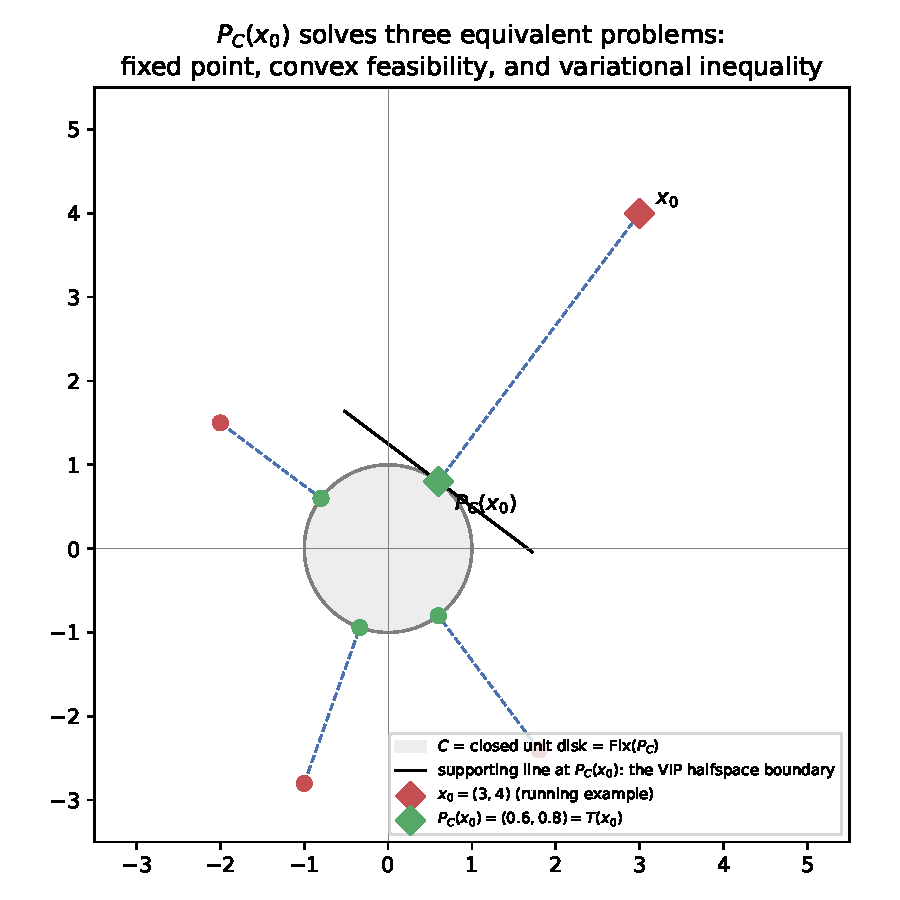
\includegraphics[width=0.46\textwidth]{fig_projection_feasibility.pdf}

\footnotesize
The projection $P_C(x_0)$ solves three equivalent problems at once: the
\textbf{fixed point problem} for $T=P_C$ (green points are all fixed,
since $\Fix(P_C)=C$); the (trivial) \textbf{convex feasibility problem}
of finding a point in $C$; and the \textbf{variational inequality} shown
by the supporting line at $P_C(x_0)$, separating $x_0$ from the rest of
$C$.

\end{frame}

\begin{frame}{1.2(C) The Hierarchical Fixed Point Problem}

A refinement: among possibly \emph{many} fixed points of $T$, select the
one closest to (or otherwise ``preferred by'') a second nonexpansive map
$V$.

\begin{block}{Hierarchical variational inequality problem, HVIP}
Let $T,V:C\to C$ be nonexpansive. Find $x^*\in\Fix(T)$ such that
\[
  \langle x^*-V x^*,\,y-x^*\rangle \ge 0 \qquad \text{for all } y\in\Fix(T).
\]
Equivalently, $x^*=P_{\Fix(T)}Vx^*$ -- i.e., $x^*$ is a fixed point of the
(again nonexpansive) map $P_{\Fix(T)}V$, where $P_K$ denotes metric
projection onto a closed convex set $K$.
\end{block}

\begin{itemize}
  \item \textbf{If $V=\Id$}: the HVIP solution set is exactly $\Fix(T)$
    (no extra selection is imposed).
  \item \textbf{If $V\equiv u$ (a constant map)}: HVIP becomes ``find the
    fixed point of $T$ closest to $u$,''
    $x^*=P_{\Fix(T)}u=\operatorname*{argmin}_{x\in\Fix(T)}\tfrac12\|u-x\|^2$
    -- exactly the target of the Halpern iteration (Section 1.1(D))!
  \item \textbf{As an equilibrium problem}: with $C=\Fix(T)$ and
    $f(x,y)=\langle(\Id-V)x,\,y-x\rangle$, HVIP is exactly EP for this
    $f$.
\end{itemize}

\end{frame}

\begin{frame}[allowframebreaks]{1.2(D) The Integral Equation}

Integral and integro-differential equations form another large class of
operator equations naturally reformulated as fixed point problems.

\begin{block}{A general integral equation (Eq.\ 1.22)}
\[
  y(x) = f(x) + \int_0^1 K(x,s,y(x),y(s))\,ds \qquad \text{for all } x\in[0,1].
\]
\begin{itemize}
  \item $K$: the \emph{kernel} of the equation; $f$: a given ``source''
    function; $y$: the unknown function.
\end{itemize}
\end{block}

Three important special cases:
\begin{itemize}
  \item \textbf{Radiation transfer}: $y(x)=1+\int_0^1
    \frac{s\,y(s)y(x)}{s+x}\varphi(s)\,ds$, with $\varphi$ given.
  \item \textbf{Urysohn equation}: $y(x)=1+\int_0^1 K(x,s,y(s))\,ds$.
  \item \textbf{Nonlinear Fredholm integral equation} (Eq.\ 1.23):
    $y(x)=f(x)+\lambda\int_0^1 K(x,s,y(s))\,ds$, with $\lambda\in\R$
    given.
\end{itemize}

\framebreak

\begin{block}{Turning Eq.\ 1.23 into a fixed point problem}
\textbf{Assumptions:} $K:[0,1]\times[0,1]\times I\to\R$ continuous and
bounded; $K$ is $L$-Lipschitz in its third variable
($|K(x,s,z_1)-K(x,s,z_2)|\le L|z_1-z_2|$); $f:[0,1]\to\R$ continuous;
$\lambda\in\R$ given; the unknown $\varphi:[0,1]\to I$ is continuous.

Let $X=C[0,1]$ with the Chebyshev metric
$d(\varphi_1,\varphi_2)=\max_{x\in[0,1]}|\varphi_1(x)-\varphi_2(x)|$ (a
complete metric space), and define, for $\varphi\in X$,
\[
  (T\varphi)(x) = f(x) + \lambda\int_0^1 K(x,s,\varphi(s))\,ds \qquad (\text{Eq. } 1.24).
\]
\begin{itemize}
  \item $T$ maps $X$ into itself (continuity of $K,f$ gives continuity of
    $T\varphi$), so Eq.\ 1.23 is equivalent to the fixed point problem
    $\varphi=T(\varphi)$.
\end{itemize}
\end{block}

\framebreak

\begin{itemize}
  \item One can show $T$ is $L|\lambda|$-Lipschitz continuous.
  \item \textbf{Choosing $|\lambda|<1/L$} makes $T$ a \emph{strict
    contraction}, so the Banach contraction principle gives a unique
    fixed point -- the unique solution of Eq.\ 1.23 -- obtainable via
    plain \textbf{Picard iteration}.
  \item This is a case where the classical (contraction-based) theory
    already suffices; the nonexpansive machinery of Section 1.1 becomes
    essential only when such a Lipschitz constant is not small enough to
    guarantee $|\lambda|L<1$.
\end{itemize}

\framebreak

\begin{block}{The Volterra integral equation of the second kind (Eq.\ 1.25)}
\[
  y(x) = f(x) + \lambda\int_a^x K(x,s,y(s))\,ds \qquad \text{for all } x\in[a,b].
\]
If $K$ is Lipschitz in its third variable, Eq.\ 1.25 has a unique
continuous solution. Defining
\[
  (T\varphi)(x) = f(x)+\lambda\int_a^x K(x,s,\varphi(s))\,ds \qquad (\text{Eq. } 1.26),
\]
Eq.\ 1.25 becomes the fixed point problem $\varphi=T(\varphi)$; for
suitable parameters, $T$ is again a contraction, and Picard iteration
approximates the unique solution.
\end{block}

\end{frame}

\begin{frame}[allowframebreaks]{1.2(E) The Ordinary Differential Equation}

Even ODEs reduce to (Volterra) integral equations, hence to fixed point
problems.

\begin{block}{Initial value problem, IVP (Eq.\ 1.27)}
\[
  \begin{cases} y' = f(x,y),\\ y(x_0)=y_0.\end{cases}
\]
Equivalent Volterra integral equation:
\[
  y(x) = y_0 + \int_{x_0}^x f(s,y(s))\,ds.
\]
\end{block}

\begin{block}{Two-point boundary value problem, BVP (Eq.\ 1.28)}
\[
  \begin{cases} y''=f(x,y),\\ y(a)=A,\quad y(b)=B.\end{cases}
\]
Equivalent integral form:
\[
  y(x) = \frac{x-a}{b-a}B + \frac{b-x}{b-a}A - \int_a^b G(x,s)f(s,y(s))\,ds,
\]
where $G$ is the \emph{Green's function} (Eq.\ 1.29)
\[
  G(x,s) = \begin{cases}
    \dfrac{(s-a)(b-x)}{b-a}, & a\le s\le x\le b,\\[6pt]
    \dfrac{(x-a)(b-s)}{b-a}, & a\le x\le s\le b,
  \end{cases}
\]
associated with the homogeneous problem $y''=0$, $y(a)=0$, $y(b)=0$.
\end{block}

\framebreak

\begin{itemize}
  \item $G(x,s)$: encodes ``how much a unit forcing term at location $s$
    influences the solution's value at location $x$,'' for the simplest
    (homogeneous) version of the boundary value problem.
  \item Under standard assumptions on $f$ (continuous, Lipschitz in the
    last variable), the corresponding integral operators satisfy a
    contractive condition, so the Banach fixed point theorem -- and
    Picard iteration -- again apply directly.
  \item \textbf{Big picture for Section 1.2}: nonlinear equations,
    equilibrium/variational/game-theoretic problems, integral equations,
    and differential equations all reduce to the \emph{same} underlying
    computational primitive: find $x^*$ with $T(x^*)=x^*$. This is
    precisely why the iterative schemes of Section 1.1 are so broadly
    useful.
\end{itemize}

\end{frame}

\begin{frame}[fragile]{Python: Convex Feasibility via the Running Example's VIP Characterization}

We numerically confirm that $P_C(x_0)$ (our running example) satisfies
the variational-inequality characterization from Section 1.2(B$'$)(5):
$\langle x_0-x^*,\,y-x^*\rangle\le 0$ for \emph{every} $y\in C$.

\begin{lstlisting}
import numpy as np
def project_disk(x):
    n = np.linalg.norm(x)
    return x if n <= 1.0 else x / n

x0 = np.array([3.0, 4.0])
x_star = project_disk(x0)                # x* = P_C(x0) = (0.6, 0.8)
print("x* = P_C(x0) =", x_star)

rng = np.random.default_rng(0)           # sample y in C, check the VIP
worst = -np.inf
for _ in range(200_000):
    y = rng.uniform(-1, 1, size=2)
    if np.linalg.norm(y) > 1:            # keep only y in C
        continue
    val = np.dot(x0 - x_star, y - x_star)   # should be <= 0 always
    worst = max(worst, val)
print(f"max <x0-x*, y-x*> over sampled y in C = {worst:.6f}  (should be <= 0)")
\end{lstlisting}

\medskip
\textbf{Output (excerpt):} \texttt{x* = [0.6 0.8]}, and
\texttt{max ... = 0.000000} (attained only at $y=x^*$ itself) --
confirming numerically that $P_C(x_0)$ solves the VIP, hence the fixed
point problem for $T=P_C$, hence the (trivial) convex feasibility problem
of finding a point of $C$.

\end{frame}

%% ══════════════════════════════════════════════════════════════════════════
\section{1.3 Outline}
%% ══════════════════════════════════════════════════════════════════════════

\begin{frame}[allowframebreaks]{1.3 Outline: Roadmap of the Book}

Since its introduction in 1953, the Krasnosel'ski\u{i}--Mann iteration has
been a cornerstone of fixed point theory, with an enormous and growing
literature on its convergence in different spaces and its many variants.
Especially in the last decade, attention has focused on it as a key tool
in optimization, together with accelerations such as \emph{inertia} and
\emph{relaxation}. Here is how the rest of the book is organized.

\begin{block}{Chapter 3: The original Krasnosel'ski\u{i}--Mann iteration}
The mean iteration scheme introduced by Mann, recently extended to a
broad class of relaxed fixed point algorithms on the convex hull (or the
affine hull) of orbits. Covers Krasnosel'ski\u{i}--Mann iterations with
\emph{perturbations} and their bounded perturbation resilience, and
summarizes recent research on convergence \emph{rate}, including global
pointwise and ergodic iteration-complexity bounds.
\end{block}

\framebreak

\begin{block}{Chapter 4: Relations to operator splitting methods}
Shows how several famous operator-splitting methods can be recast as
instances of the Krasnosel'ski\u{i}--Mann iteration: the proximal point
method, the forward-backward splitting method, the backward-forward
splitting method, the Douglas--Rachford splitting method, the Davis--Yin
splitting method, and a class of primal-dual splitting methods.
\end{block}

\begin{block}{Chapter 5: The inertial Krasnosel'ski\u{i}--Mann iteration}
Recent progress on the inertial variant first introduced by Maing\'e,
especially the \emph{general} inertial Krasnosel'ski\u{i}--Mann iteration.
Focuses on the inertial parameters and presents several valid ranges for
them; also covers the alternated inertial and the online inertial
Krasnosel'ski\u{i}--Mann iterations.
\end{block}

\framebreak

\begin{block}{Chapter 6: The multi-step inertial Krasnosel'ski\u{i}--Mann iteration}
Presents its convergence analysis, including two classes of inertial
parameter sequences that do not involve the iterative sequence itself.
Introduces a general Krasnosel'ski\u{i}--Mann iteration on the affine hull
of orbits and a modified Krasnosel'ski\u{i}--Mann iteration. Applications:
multi-step inertial versions of the forward-backward, backward-forward,
Douglas--Rachford, Davis--Yin, and primal-dual splitting methods.
\end{block}

\begin{block}{Chapter 7: Choosing the relaxation parameters}
Discusses the line search method, the online choice, and the optimal
choice of relaxation parameters. Using the equivalence between fixed
point problems and variational inequality problems, presents (multi-step)
inertial Krasnosel'ski\u{i}--Mann iterations with \emph{adaptive}
relaxation parameters, and a residual algorithm exploiting the
equivalence between fixed point problems and nonlinear monotone
equations.
\end{block}

\framebreak

\begin{block}{Chapter 8 (final): Two applications}
Asynchronous parallel coordinate-update methods, and cyclic
coordinate-update algorithms. Convergence analysis and convergence rate
are presented under suitable conditions for both.
\end{block}

\textbf{In short:} Chapter 1 (this chapter) built the vocabulary and the
basic toolbox of iteration schemes; Chapters 3--8 progressively refine,
accelerate, connect, and apply the Krasnosel'ski\u{i}--Mann iteration
across the rest of the book. (Chapter 2, not previewed above, lays the
formal groundwork -- precise definitions of contractions, monotonicity,
and related operator classes referenced throughout this chapter.)

\end{frame}

%% ══════════════════════════════════════════════════════════════════════════
\section{Summary}
%% ══════════════════════════════════════════════════════════════════════════

\begin{frame}{Chapter 1 --- Key Takeaways}
\small
\begin{itemize}
  \item The \textbf{fixed point problem} ($T(x^*)=x^*$ for $T:C\to C$)
    unifies a remarkable range of computational questions; this chapter's
    job is cataloguing \emph{how to compute} such an $x^*$.
  \item \textbf{Picard iteration} ($x_{n+1}=T(x_n)$) converges for
    contractions, but can fail for merely nonexpansive maps (our
    $T=-\Id$ example: oscillates forever).
  \item \textbf{Krasnosel'ski\u{i} averaging}
    ($x_{n+1}=\tfrac12 x_n+\tfrac12 T(x_n)$, generalized to
    Krasnosel'ski\u{i}--Mann with $\lambda_n$) repairs this: on our
    running example ($T=P_C$, $x_0=(3,4)$) it converges geometrically,
    $r_0{=}5,r_1{=}3,r_2{=}2,\dots,r_6{=}1.0625\to1$.
  \item \textbf{Stronger convergence} (strong, not just weak) is bought
    via anchoring (\textbf{Halpern}), moving anchors (\textbf{viscosity}),
    regularization, or projections (\textbf{hybrid/CQ methods}) -- each
    with its own trade-offs in conditions and computational cost.
  \item \textbf{Section 1.2's big idea}: nonlinear equations (Newton's
    method), equilibrium problems (which subsume minimization, saddle
    points, Nash equilibria, variational inequalities, and
    complementarity problems), and integral/differential equations all
    reduce to the \emph{same} fixed point primitive -- and our running
    example's projection $P_C(x_0)$ instantiates this concretely as a
    fixed point / convex feasibility / variational inequality problem all
    at once.
  \item The rest of the book (Chapters 2--8) builds outward from these
    definitions: formal groundwork (Ch.\ 2), the Krasnosel'ski\u{i}--Mann
    iteration in depth and its splitting-method relatives (Ch.\ 3--4),
    inertial acceleration (Ch.\ 5--6), adaptive relaxation (Ch.\ 7), and
    parallel/cyclic coordinate-update applications (Ch.\ 8).
\end{itemize}

\end{frame}

\end{document}
